\documentclass[manuscript,nonacm]{acmart}
\usepackage{float}
\usepackage{subcaption}
\AtBeginDocument{%
  \providecommand\BibTeX{{Bib\TeX}}}

% -------------------------
% Metadaten (ANPASSEN)
% -------------------------

\title{Analysis of Spatio-Temmporal Data - Final Report (WiSe 2025/26)}

\author{Lukas Räuschel}
\email{l.raeuschel@uni-muenster.de}
\affiliation{%
  \institution{University of Münster}
  \city{Münster}
  \country{Germany}
}

\setcopyright{none}
\copyrightyear{2026}
\acmYear{2026}
\acmDOI{}

\settopmatter{printacmref=false}
\renewcommand\footnotetextcopyrightpermission[1]{}

% Bei mehreren Autoren einfach kopieren

\renewcommand{\shortauthors}{Räuschel}

% -------------------------
% Abstract
% -------------------------

\begin{document}

\maketitle

% -------------------------
% Inhalt
% -------------------------


\section{Introduction}
    Air pollution represents a major environmental and public health challenge in highly urbanized regions. Hong Kong regularly experiences elevated air pollution levels due to dense urban structures, intensive traffic, and regional atmospheric transport processes.

    The Air Quality Health Index (AQHI), provided by the Hong Kong Environmental Protection Department, is a health risk-based air pollution indicator estimating short-term health risks associated with atmospheric pollution.

    The AQHI is calculated from the combined health effects of four major pollutants: Ozone (O\textsubscript{3}), Nitrogen Dioxide (NO\textsubscript{2}), Sulphur Dioxide (SO\textsubscript{2}), and particulate matter (PM\textsubscript{10} / PM\textsubscript{2.5}). The index is derived from 3-hour moving average pollutant concentrations and represents additional health risk percentages based on hospital admission statistics.

    Further information about the AQHI calculation methodology is provided by the Hong Kong Environmental Protection Department:
    \url{https://www.aqhi.gov.hk/en/what-is-aqhi/faqs.html}

    The objective of this project is to analyze the spatio-temporal distribution of AQHI values in Hong Kong and to explore temporal trends as well as spatial variability between monitoring stations. In addition, an interactive dashboard was developed to communicate the results and allow flexible exploration of the data.

    The workflow integrates multi-year hourly AQHI measurements, spatial interpolation techniques, and interactive visualization tools within a reproducible analysis pipeline implemented in R.

\section{Personas and User Stories}
    To ensure the analysis and dashboard development are user-centered and address real-world needs, two personas were defined representing typical stakeholders concerned with air quality in Hong Kong. These personas guide the analytical approach and visualization design, ensuring the final product delivers meaningful insights to different user groups.

    \subsection{Persona 1: Elementary School Teacher – Anna}
    
    Anna is a 29-year-old elementary school teacher living in Hong Kong. She works at a school located near a busy main road where children frequently play outside. Anna has observed that some students complain about headaches or discomfort on certain days, raising her concerns about the impact of air pollution on the health and well-being of her students. As a teacher, she wants to understand seasonal variations in air pollution so she can plan outdoor activities during safer months. Furthermore, as a person concerned about children's well-being, she wants to understand how air pollution has developed over recent years to see whether the situation is improving or worsening.
    
    \subsection{Persona 2: Data Analyst with Asthma – John}
    
    John is a 34-year-old data analyst working in Hong Kong. Although he spends most of his time working indoors, John has asthma, making him particularly sensitive to air quality. Long-term exposure to polluted air affects his breathing and overall health. He is interested in analyzing long-term trends in air pollution to make informed decisions about where to live and how to manage his health condition. As a data analyst, he wants to analyze long-term air pollution trends in Hong Kong to understand how conditions have changed and may continue to change in the future. As a resident with asthma, he wants to compare pollution levels across different districts so he can evaluate which areas might be healthier to live in.

    These personas and their associated user stories inform the analytical focus of this project, emphasizing the need for temporal trend analysis, seasonal pattern identification, and spatial comparison of air quality across Hong Kong's monitoring stations.

\section{Study Area}
    Hong Kong is a Special Administrative Region of China located on the southern coast at the mouth of the Pearl River Delta. The territory covers approximately 1,104 km\textsuperscript{2} and comprises Hong Kong Island, Kowloon Peninsula, the New Territories, and over 200 offshore islands. With a population of approximately 7.5 million inhabitants, Hong Kong represents one of the most densely populated metropolitan regions globally.

    The region is characterized by complex topography, featuring mountainous terrain interspersed with urban development concentrated in coastal lowlands and valleys. This topographic complexity significantly influences local atmospheric circulation patterns and pollutant dispersion.

    Air quality in Hong Kong is influenced by both local emission sources (vehicular traffic, marine vessels, power generation, and commercial activities) and regional atmospheric transport from the industrialized Pearl River Delta region. The combination of high-density urban development, intensive transportation infrastructure, and regional pollution sources creates a complex air quality environment requiring comprehensive spatial and temporal analysis \cite{hk_epd_air_overview}.

    The Hong Kong Environmental Protection Department operates an air quality monitoring network consisting of general monitoring stations distributed across urban, suburban, and rural environments, as well as roadside stations positioned near major traffic corridors \cite{hk_map_source}. This monitoring infrastructure enables spatial comparison of air pollution levels across different land-use types and exposure environments. Figure \ref{fig:study_area} illustrates the geographic location of Hong Kong and the spatial distribution of monitoring stations used in this analysis.

\begin{figure}[htbp]
    \centering
    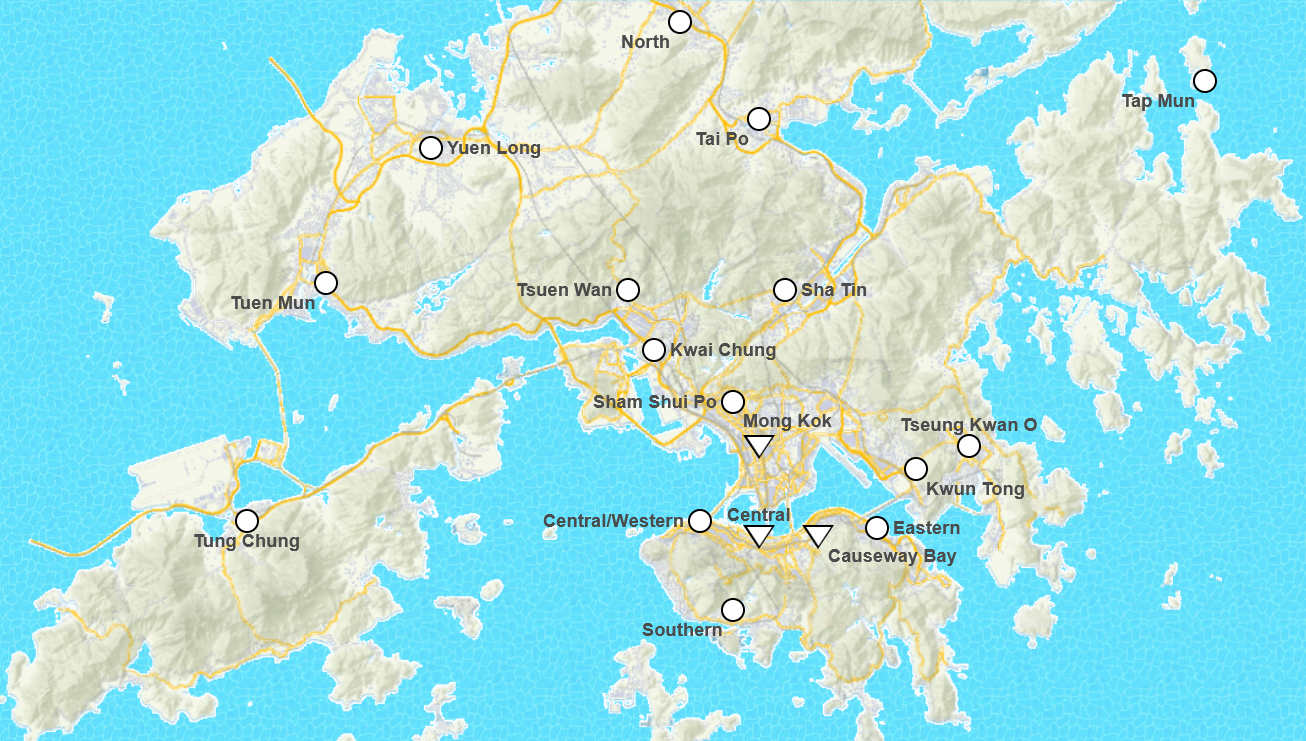
\includegraphics[width=0.7\textwidth]{figures/study_area.png}
    \caption{Geographic location of Hong Kong and spatial distribution of AQHI monitoring stations \cite{hk_map_source}.}
    \label{fig:study_area}
\end{figure}

\section{Data Sources}

    This project integrates multiple open datasets related to air quality monitoring and spatial reference information for Hong Kong. The datasets were obtained from official government sources and provide both temporal measurements of air pollution and spatial information required for geostatistical analysis and visualization.

    \subsection{Past AQHI Observations}

        Hourly observations of the AQHI were obtained from the Hong Kong Environmental Protection Department (EPD). The dataset is publicly available through the AQHI data portal and is provided as monthly CSV files containing hourly AQHI values for each monitoring station across Hong Kong.

        The temporal resolution of the dataset is hourly, allowing for detailed analysis of short-term air quality variations as well as aggregation to daily, monthly, and annual levels. For this project, all available data from January 2021 to December 2025 were collected and combined into a single dataset. The data were downloaded from the official AQHI archive \cite{hk_epd_past_aqhi}.

    \subsection{Monitoring Station Locations}

        Spatial information on the locations of the AQHI monitoring stations was obtained from the Hong Kong Environmental Protection Department website. The geographic coordinates of all monitoring stations were manually compiled from the official EPD monitoring network portal and used to create a spatial dataset. Using QGIS, a shapefile was created containing all monitoring station locations with their corresponding coordinates and identifiers.

        These spatial point data were required to link the hourly AQHI observations to their geographic positions and to enable spatial interpolation methods such as Kriging and inverse distance weighting (IDW). The manually created shapefile provides a precise spatial representation of the monitoring network, enabling detailed spatial analysis across Hong Kong's urban, suburban, and roadside environments.

    \subsection{Administrative Boundaries}

        Administrative boundary data for Hong Kong were obtained from the Hong Kong Government Open Data Portal. The dataset is provided in GeoJSON format and contains polygon geometries representing the administrative districts of Hong Kong.

        These boundary data were primarily used for spatial visualization and for defining the spatial extent of the interpolation grid used in the geostatistical analysis. The dataset ensures that all spatial outputs are constrained to the geographic extent of Hong Kong. Further details and access to the dataset are provided through the Hong Kong Open Data Portal \cite{hk_boundaries}.
\newpage
\section{Methodology}
    The analysis of spatio-temporal air pollution data in Hong Kong was conducted following a structured methodology that integrates data preparation, exploratory analysis, spatial interpolation, and interactive visualization. This section describes the technical approaches and computational methods employed at each stage of the analysis.

    \subsection{Data Preparation}
    
        The data preparation phase focused on the structured integration of raw AQHI observations and spatial reference data. Monthly CSV files containing hourly AQHI measurements for the period 2021–2025 were imported and consolidated using R. Data processing was primarily performed using the tidyverse ecosystem, while temporal variables were generated using the \texttt{lubridate} package.

        The raw AQHI files required several preprocessing steps due to their semi-structured format. Header metadata lines were removed during import, and all columns were initially read as character variables to avoid type inconsistencies across files. Subsequently, non-numeric symbols (e.g., asterisks used as quality flags) were removed and AQHI values were converted to numeric format.

        Missing date entries in the original tables were corrected using forward filling to reconstruct complete time stamps. A unified datetime variable was then created from the date and hour fields, from which additional temporal attributes such as year, month, and calendar date were derived.\\
        Because the original dataset is provided in wide format with one column per monitoring station, the dataset was transformed into a long structure using pivot operations. This format is required for both temporal aggregation and spatial analysis.

        Spatial reference information for AQHI monitoring stations was imported from the official EPD shapefile using the \texttt{sf} package. The AQHI observations were then linked to station geometries through attribute joins, resulting in a spatially enabled dataset containing hourly observations for all monitoring stations.

        All yearly datasets were subsequently merged into a single spatio-temporal dataset and stored in RDS format to enable efficient reuse in the dashboard and spatial interpolation workflows.

    \subsection{Spatial Interpolation Methods}

        To generate continuous air quality surfaces from the discrete AQHI observations, three spatial interpolation approaches were applied: Inverse Distance Weighting (IDW) and two variants of Ordinary Kriging. The interpolation was performed for multiple temporal aggregations, including hourly, monthly, and annual averages.

        IDW is a deterministic method in which the influence of each monitoring station decreases with distance. AQHI values at unsampled locations are computed as a weighted average of nearby stations, with weights inversely proportional to distance squared (\texttt{idp = 2.0}). This method provides a simple yet effective way to estimate continuous air quality surfaces from irregularly spaced measurements.

        Ordinary Kriging was applied in two ways. In the first approach, a variogram was fitted automatically to the observed AQHI values at the monitoring stations using the empirical variogram and the \texttt{fit.variogram} function from the \texttt{gstat} package. This procedure estimates the spatial structure of the data and determines the sill, range, and nugget parameters for Kriging. In the second approach, a manual variogram model was constructed based on the observed variance of the AQHI measurements and the median distance between stations. The manual model specified a spherical variogram with 70\% of the observed variance as the partial sill, 30\% as the nugget, and a range equal to the median inter-station distance. Both Kriging approaches produce unbiased predictions and quantify the associated estimation uncertainty.

        Prior to interpolation, monitoring station coordinates were projected to a suitable metric coordinate reference system to ensure accurate distance computations. A uniform grid with 500\,m spacing covering the Hong Kong territory was generated to serve as the target locations for interpolation. For each temporal aggregation (hour, month, year), AQHI measurements were averaged per station and projected onto the grid using the three interpolation methods. The resulting raster surfaces were saved in GeoTIFF format for subsequent spatial visualization and analysis. Missing temporal periods were tracked and documented to ensure completeness and transparency of the spatial analysis.

    \section{Final Product: Interactive Dashboard}

        An interactive web-based dashboard was developed using the \texttt{Shiny} framework in R to enable flexible and user-centered exploration of spatio-temporal patterns of the Air Quality Health Index (AQHI) across Hong Kong. The application is based on reactive programming principles, allowing visualizations and maps to update dynamically in response to user selections without requiring page reloads. This approach supports intuitive exploration while maintaining computational efficiency.

        The dashboard integrates multiple data sources generated during the preprocessing and spatial analysis workflow. Preprocessed AQHI observations are stored in RDS format and loaded at runtime for temporal analysis, while administrative boundary geometries are imported from shapefiles to provide geographic context. Spatial interpolation outputs are stored as precomputed GeoTIFF raster layers, which are dynamically loaded depending on the selected interpolation method and temporal aggregation level. Reactive filtering is applied to the tabular AQHI dataset based on user-defined parameters such as monitoring station, year, and month, and temporal aggregations are computed on-the-fly for visualization.

        An introductory \emph{About} section provides contextual information for end users by describing the AQHI metric, including its scale, health risk categories, and calculation principles. In addition, this section documents key dataset characteristics such as the number of monitoring stations, total hourly observations, temporal coverage from 2021 to 2025, and overall data completeness. The analytical workflow and implemented interpolation methods are also briefly summarized to ensure transparency regarding the data processing pipeline.

        Temporal dynamics of air quality are explored in the \emph{Trend Analysis} component, where users can examine daily AQHI developments for individual monitoring stations or aggregated across all stations (Figure \ref{fig:dashboard_trend_analysis}). Filtering options allow selection of specific years and months, with the possibility to analyze full-year patterns. Interactive time series visualizations are implemented using \texttt{plotly}, enabling zooming and hovering for detailed inspection. When a single month is selected, markers emphasize individual daily observations, whereas annual selections are represented as continuous lines to highlight long-term structure. An optional reference line representing the mean across all stations allows direct comparison between local and territory-wide conditions. To maintain spatial awareness, monitoring station locations are simultaneously displayed on a Leaflet map, with the selected station visually highlighted.

        Complementing the long-term perspective, the \emph{Hourly Analysis} component focuses on intra-day variability (Figure \ref{fig:dashboard_hourly_analysis}). AQHI observations are grouped by hour of the day and averaged across the selected temporal window to produce a 24-hour profile. This representation enables identification of typical diurnal pollution patterns and potential peak exposure periods. Visualization design and filtering logic follow the structure of the trend analysis module, ensuring consistent interaction behavior across dashboard components while shifting the temporal focus from dates to hourly cycles.

        Spatial patterns of air quality are presented in the \emph{Spatial Analysis} component through interpolated AQHI surfaces displayed on interactive Leaflet maps (Figure \ref{fig:dashboard_spatial_analysis}). Users can select among three interpolation outputs generated during the analysis workflow: Kriging based on automatically fitted variogram parameters, Kriging using manually defined variogram parameters, and Inverse Distance Weighting (IDW). In addition, temporal aggregation levels can be switched between monthly, annual, and hourly averages. Based on these selections, the dashboard dynamically constructs the corresponding file path and loads the appropriate raster dataset using the \texttt{stars} package. Raster layers are rendered with partial transparency to maintain visibility of monitoring stations and basemap tiles.\\
        Two legend modes are available: a categorical mode aligned with official AQHI risk classes and a continuous mode scaled to the actual raster value range. Summary statistics, including minimum, maximum, and mean AQHI values, are calculated directly from raster pixels and displayed to support interpretation.

        Throughout the application, performance and usability considerations guided the implementation. Efficient storage formats, including RDS for tabular data and GeoTIFF for raster outputs, reduce loading times, while reactive programming ensures that only affected components are recalculated after user interaction. Interactive visualization features such as hover tooltips and dynamic legends further enhance interpretability. The overall dashboard structure supports different user perspectives, enabling both detailed temporal exploration and spatial comparison of air quality conditions across Hong Kong.

        \begin{figure}[H]
            \centering
            \begin{subfigure}[b]{0.32\textwidth}
                \centering
                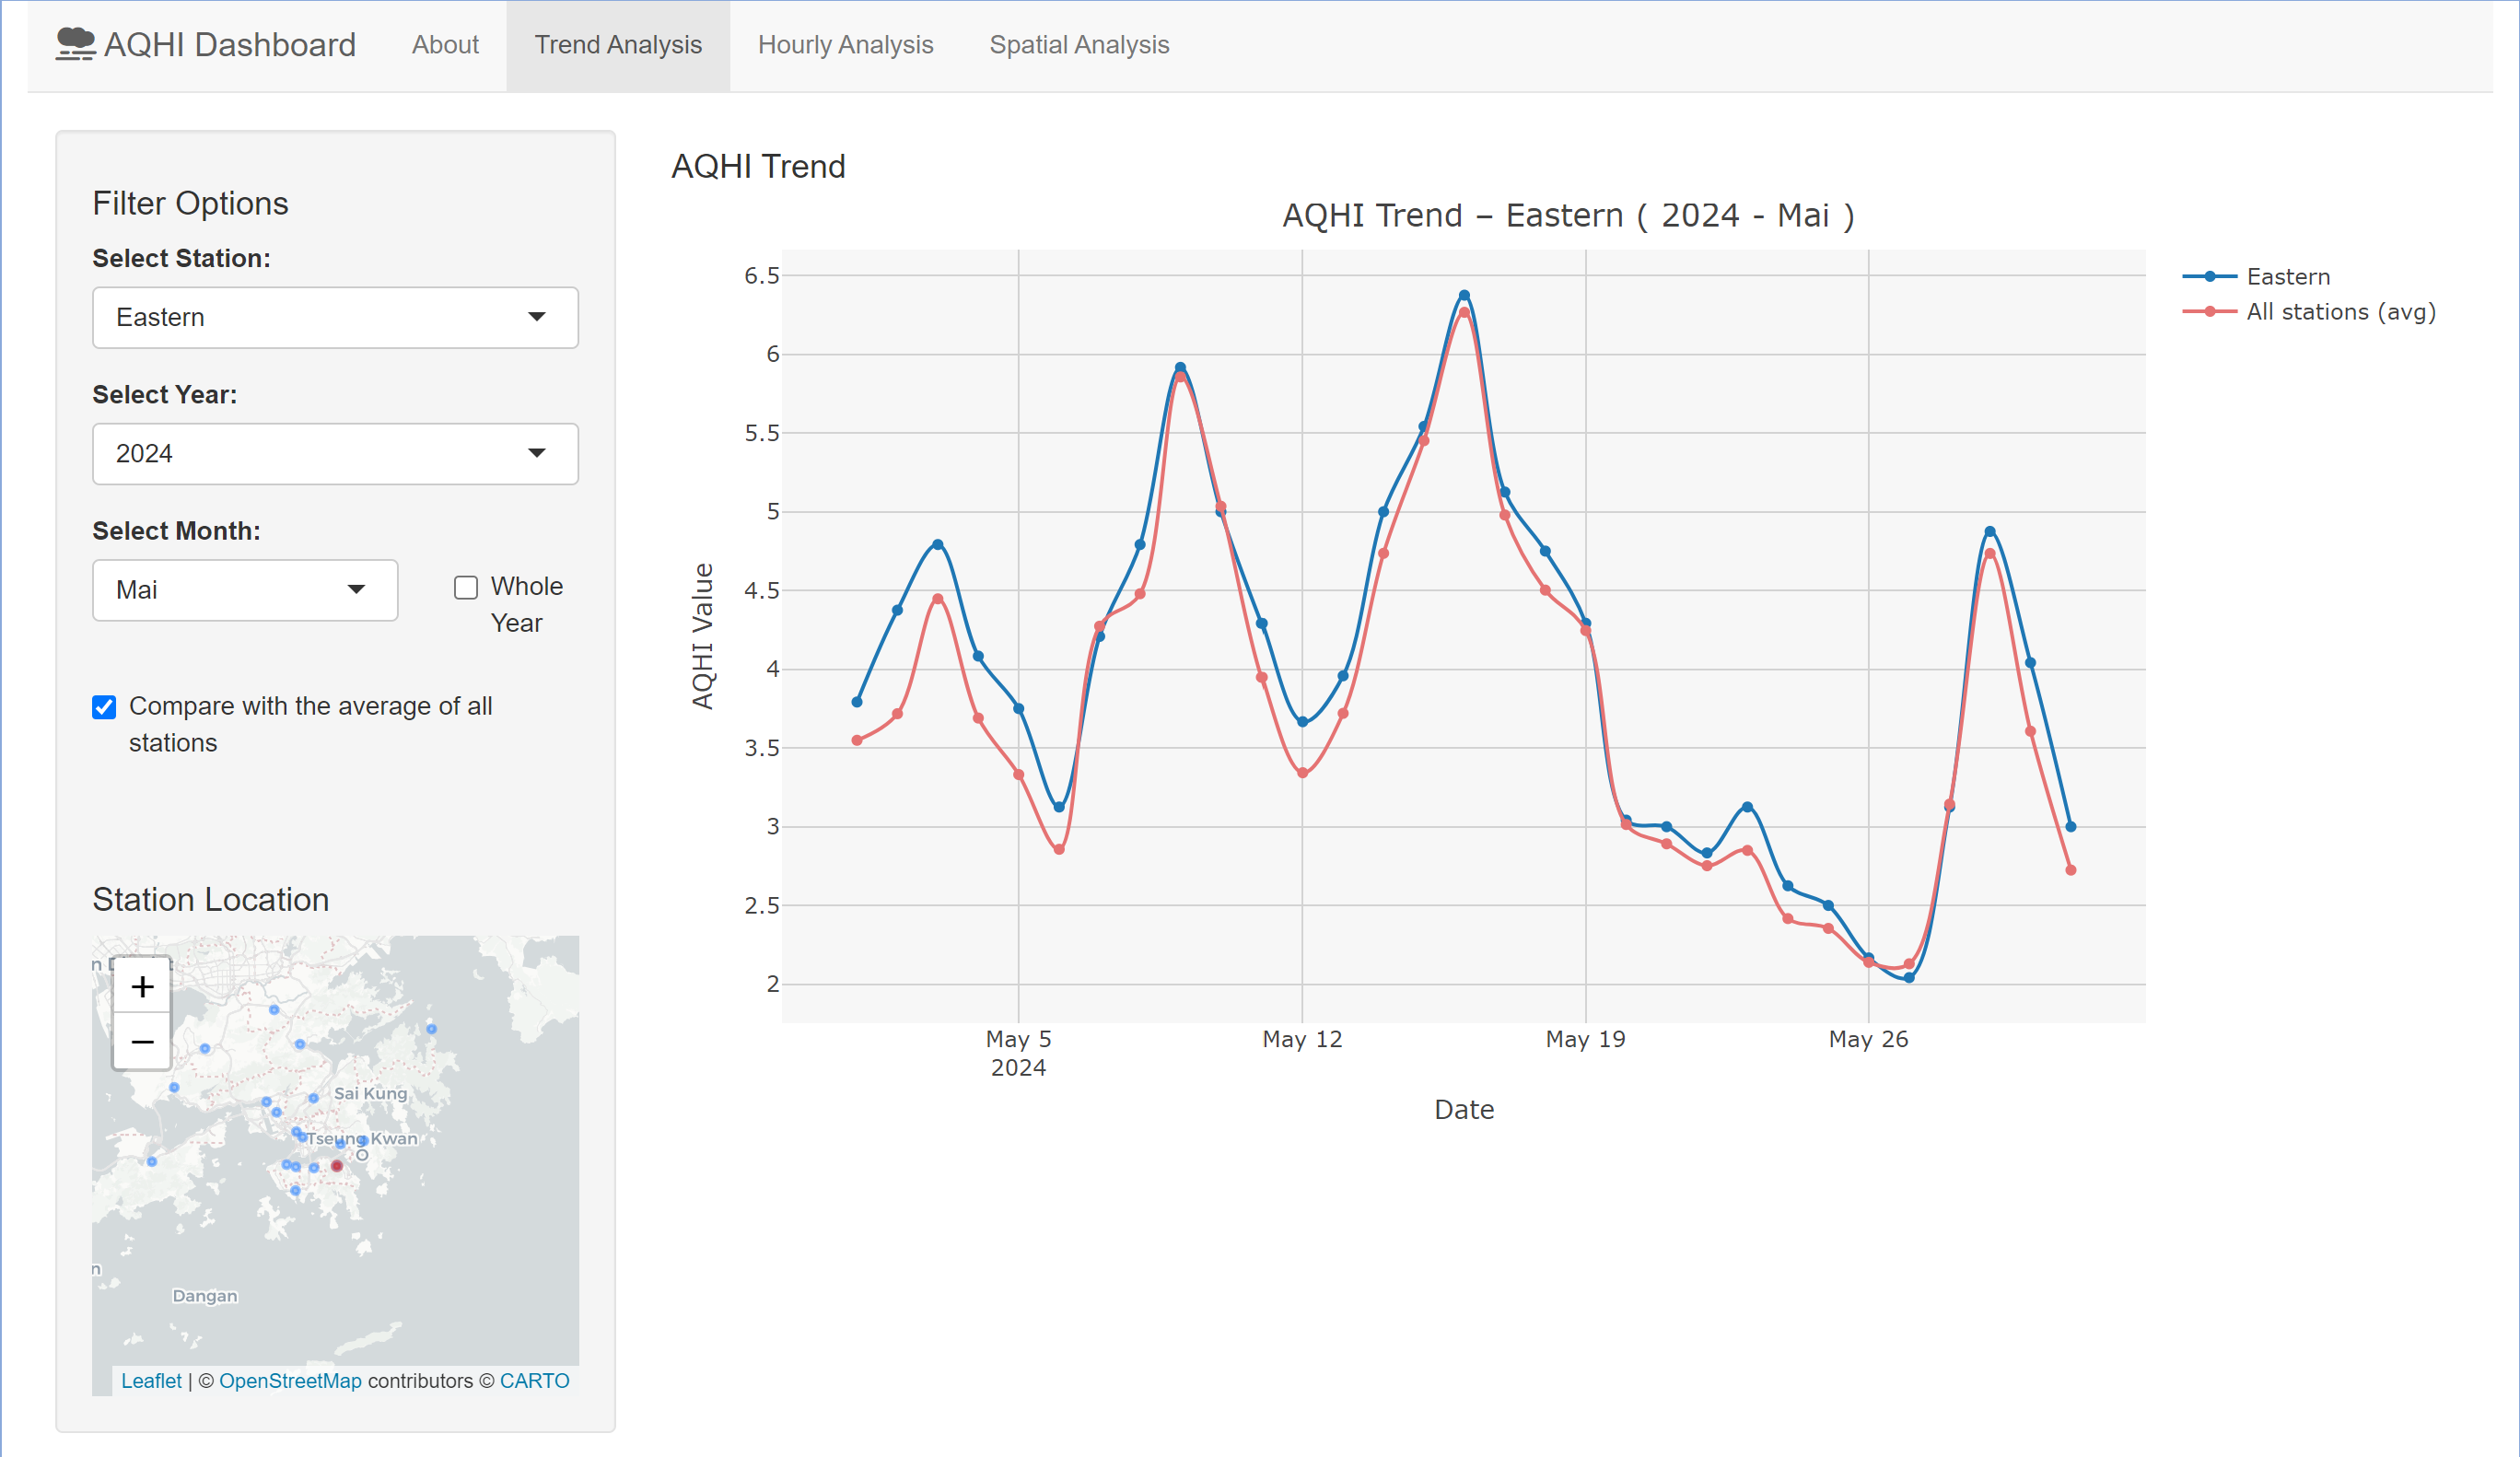
\includegraphics[width=\textwidth]{figures/trend analysis.png}
                \caption{Trend Analysis: Daily AQHI time series.}
                \label{fig:dashboard_trend_analysis}
            \end{subfigure}
            \hfill
            \begin{subfigure}[b]{0.32\textwidth}
                \centering
                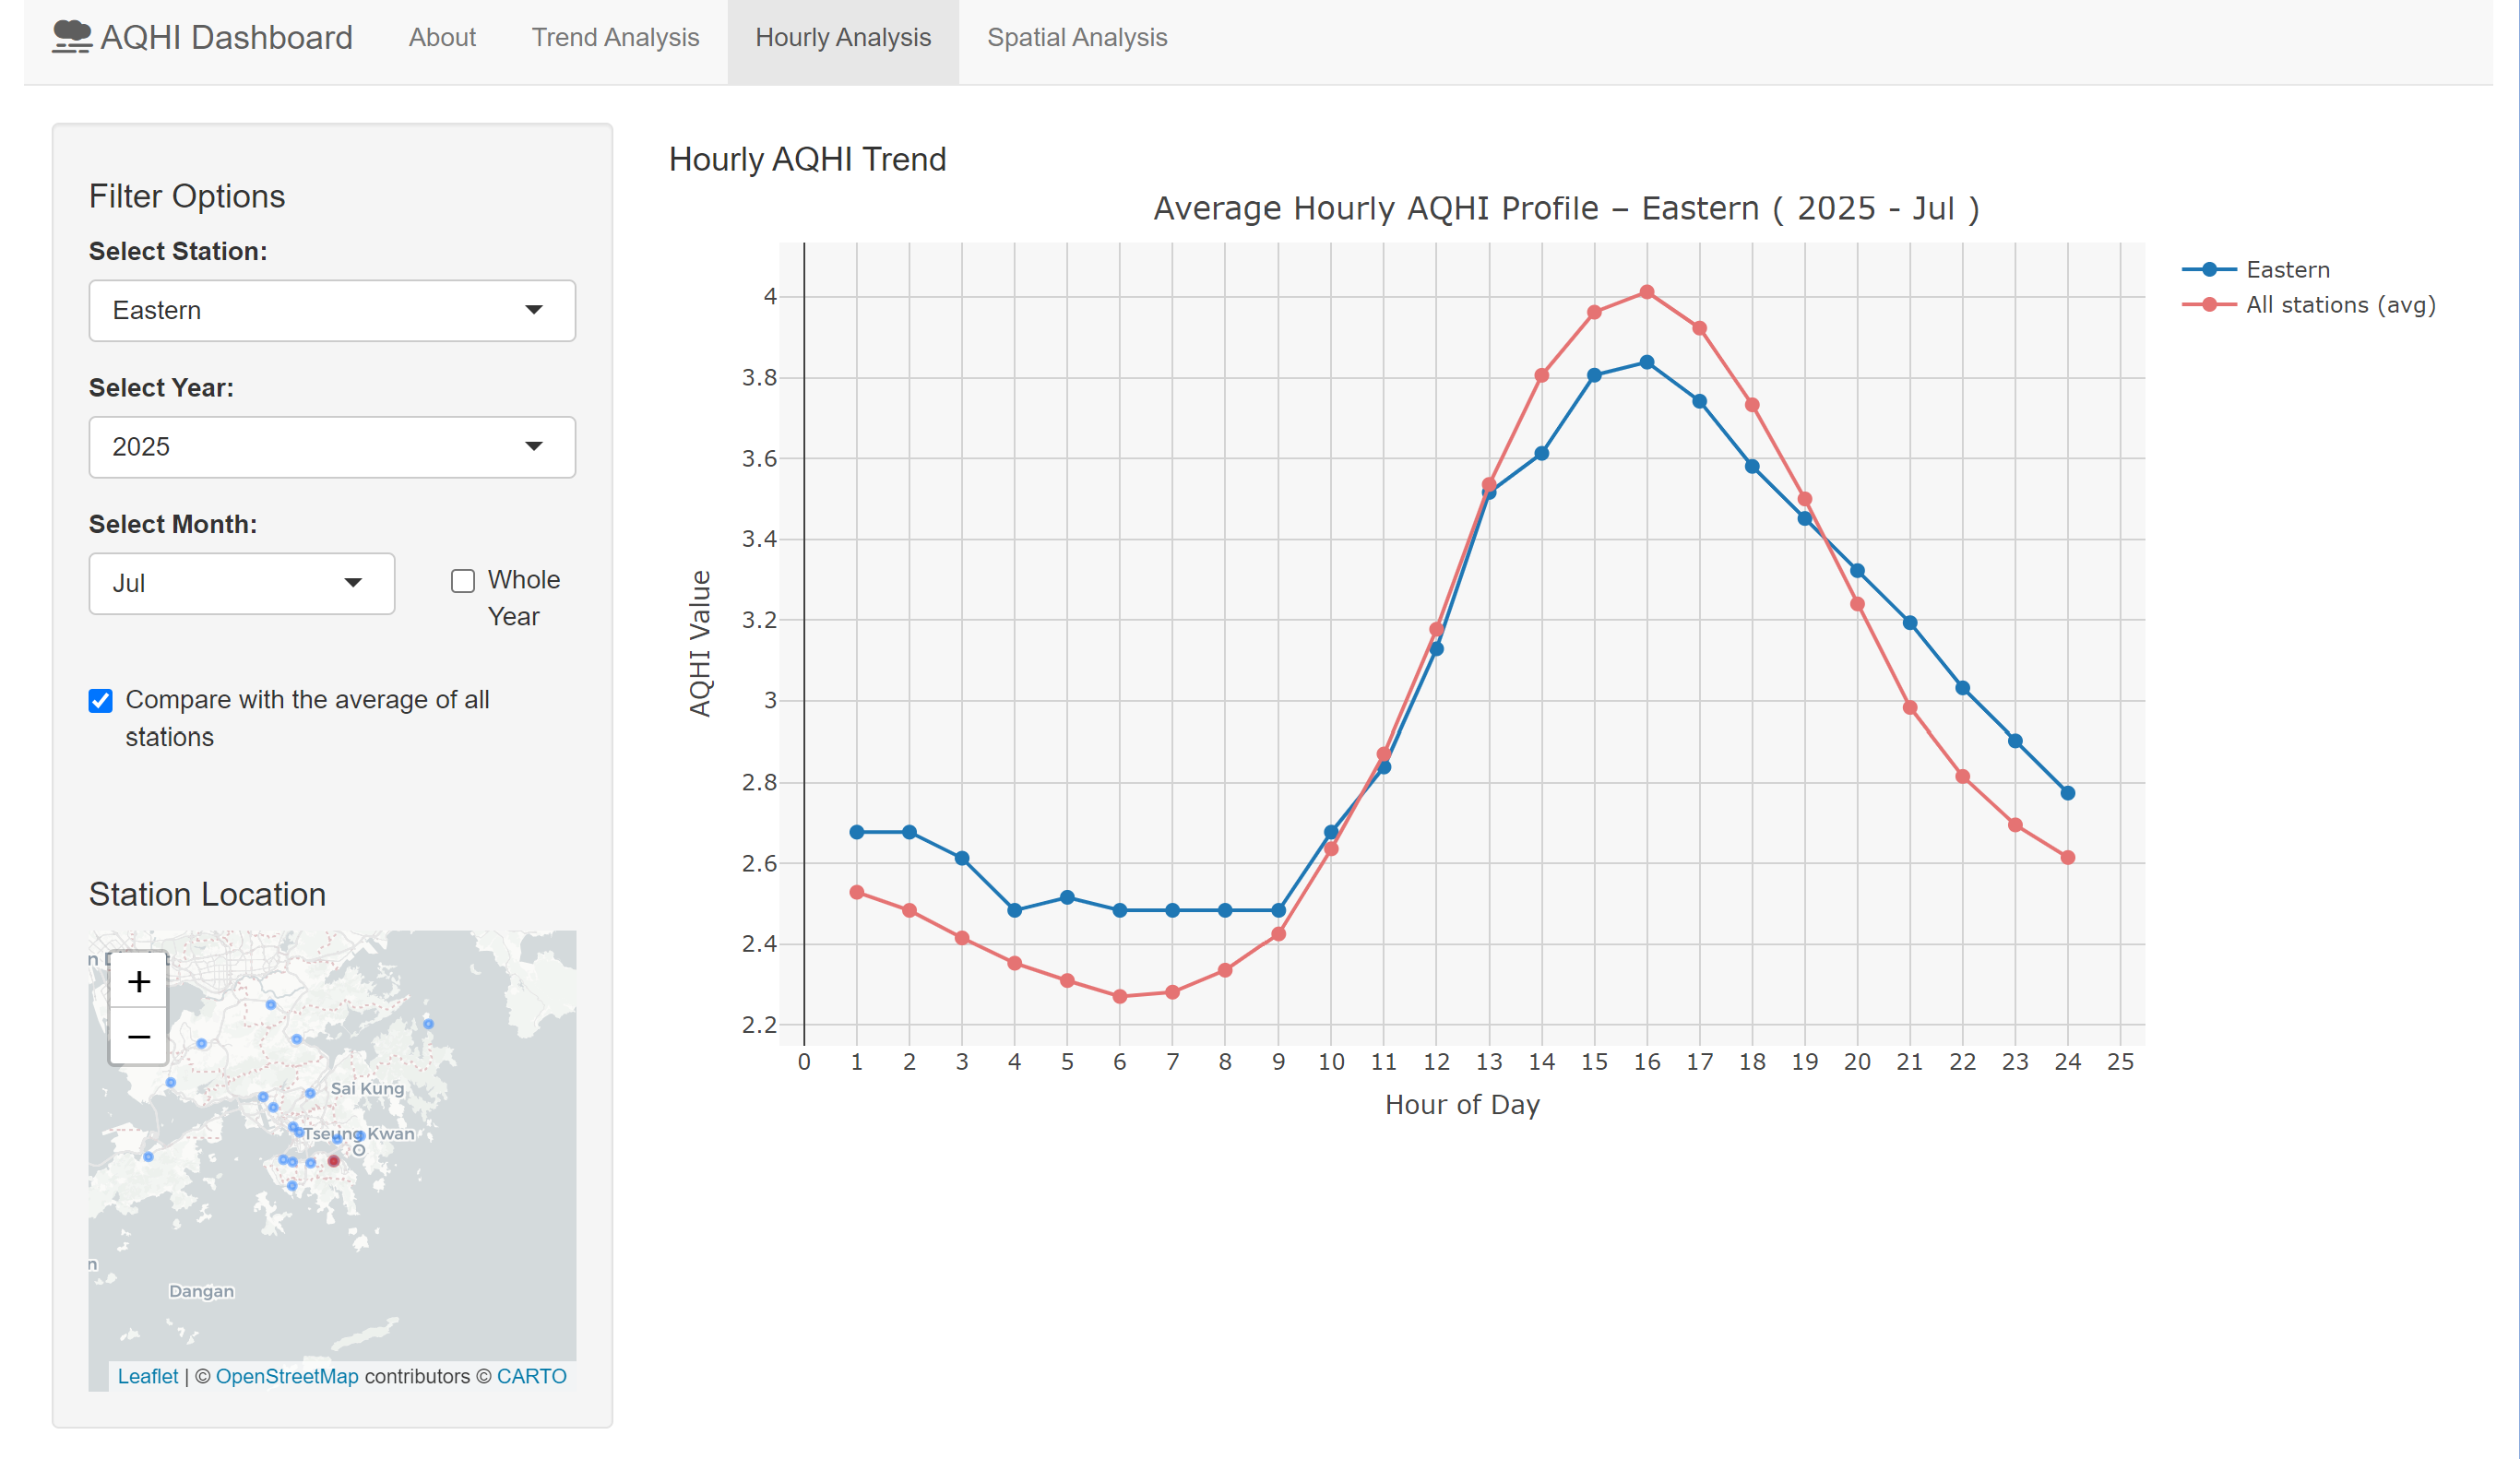
\includegraphics[width=\textwidth]{figures/hourly analysis.png}
                \caption{Hourly Analysis: 24-hour diurnal profile.}
                \label{fig:dashboard_hourly_analysis}
            \end{subfigure}
            \hfill
            \begin{subfigure}[b]{0.32\textwidth}
                \centering
                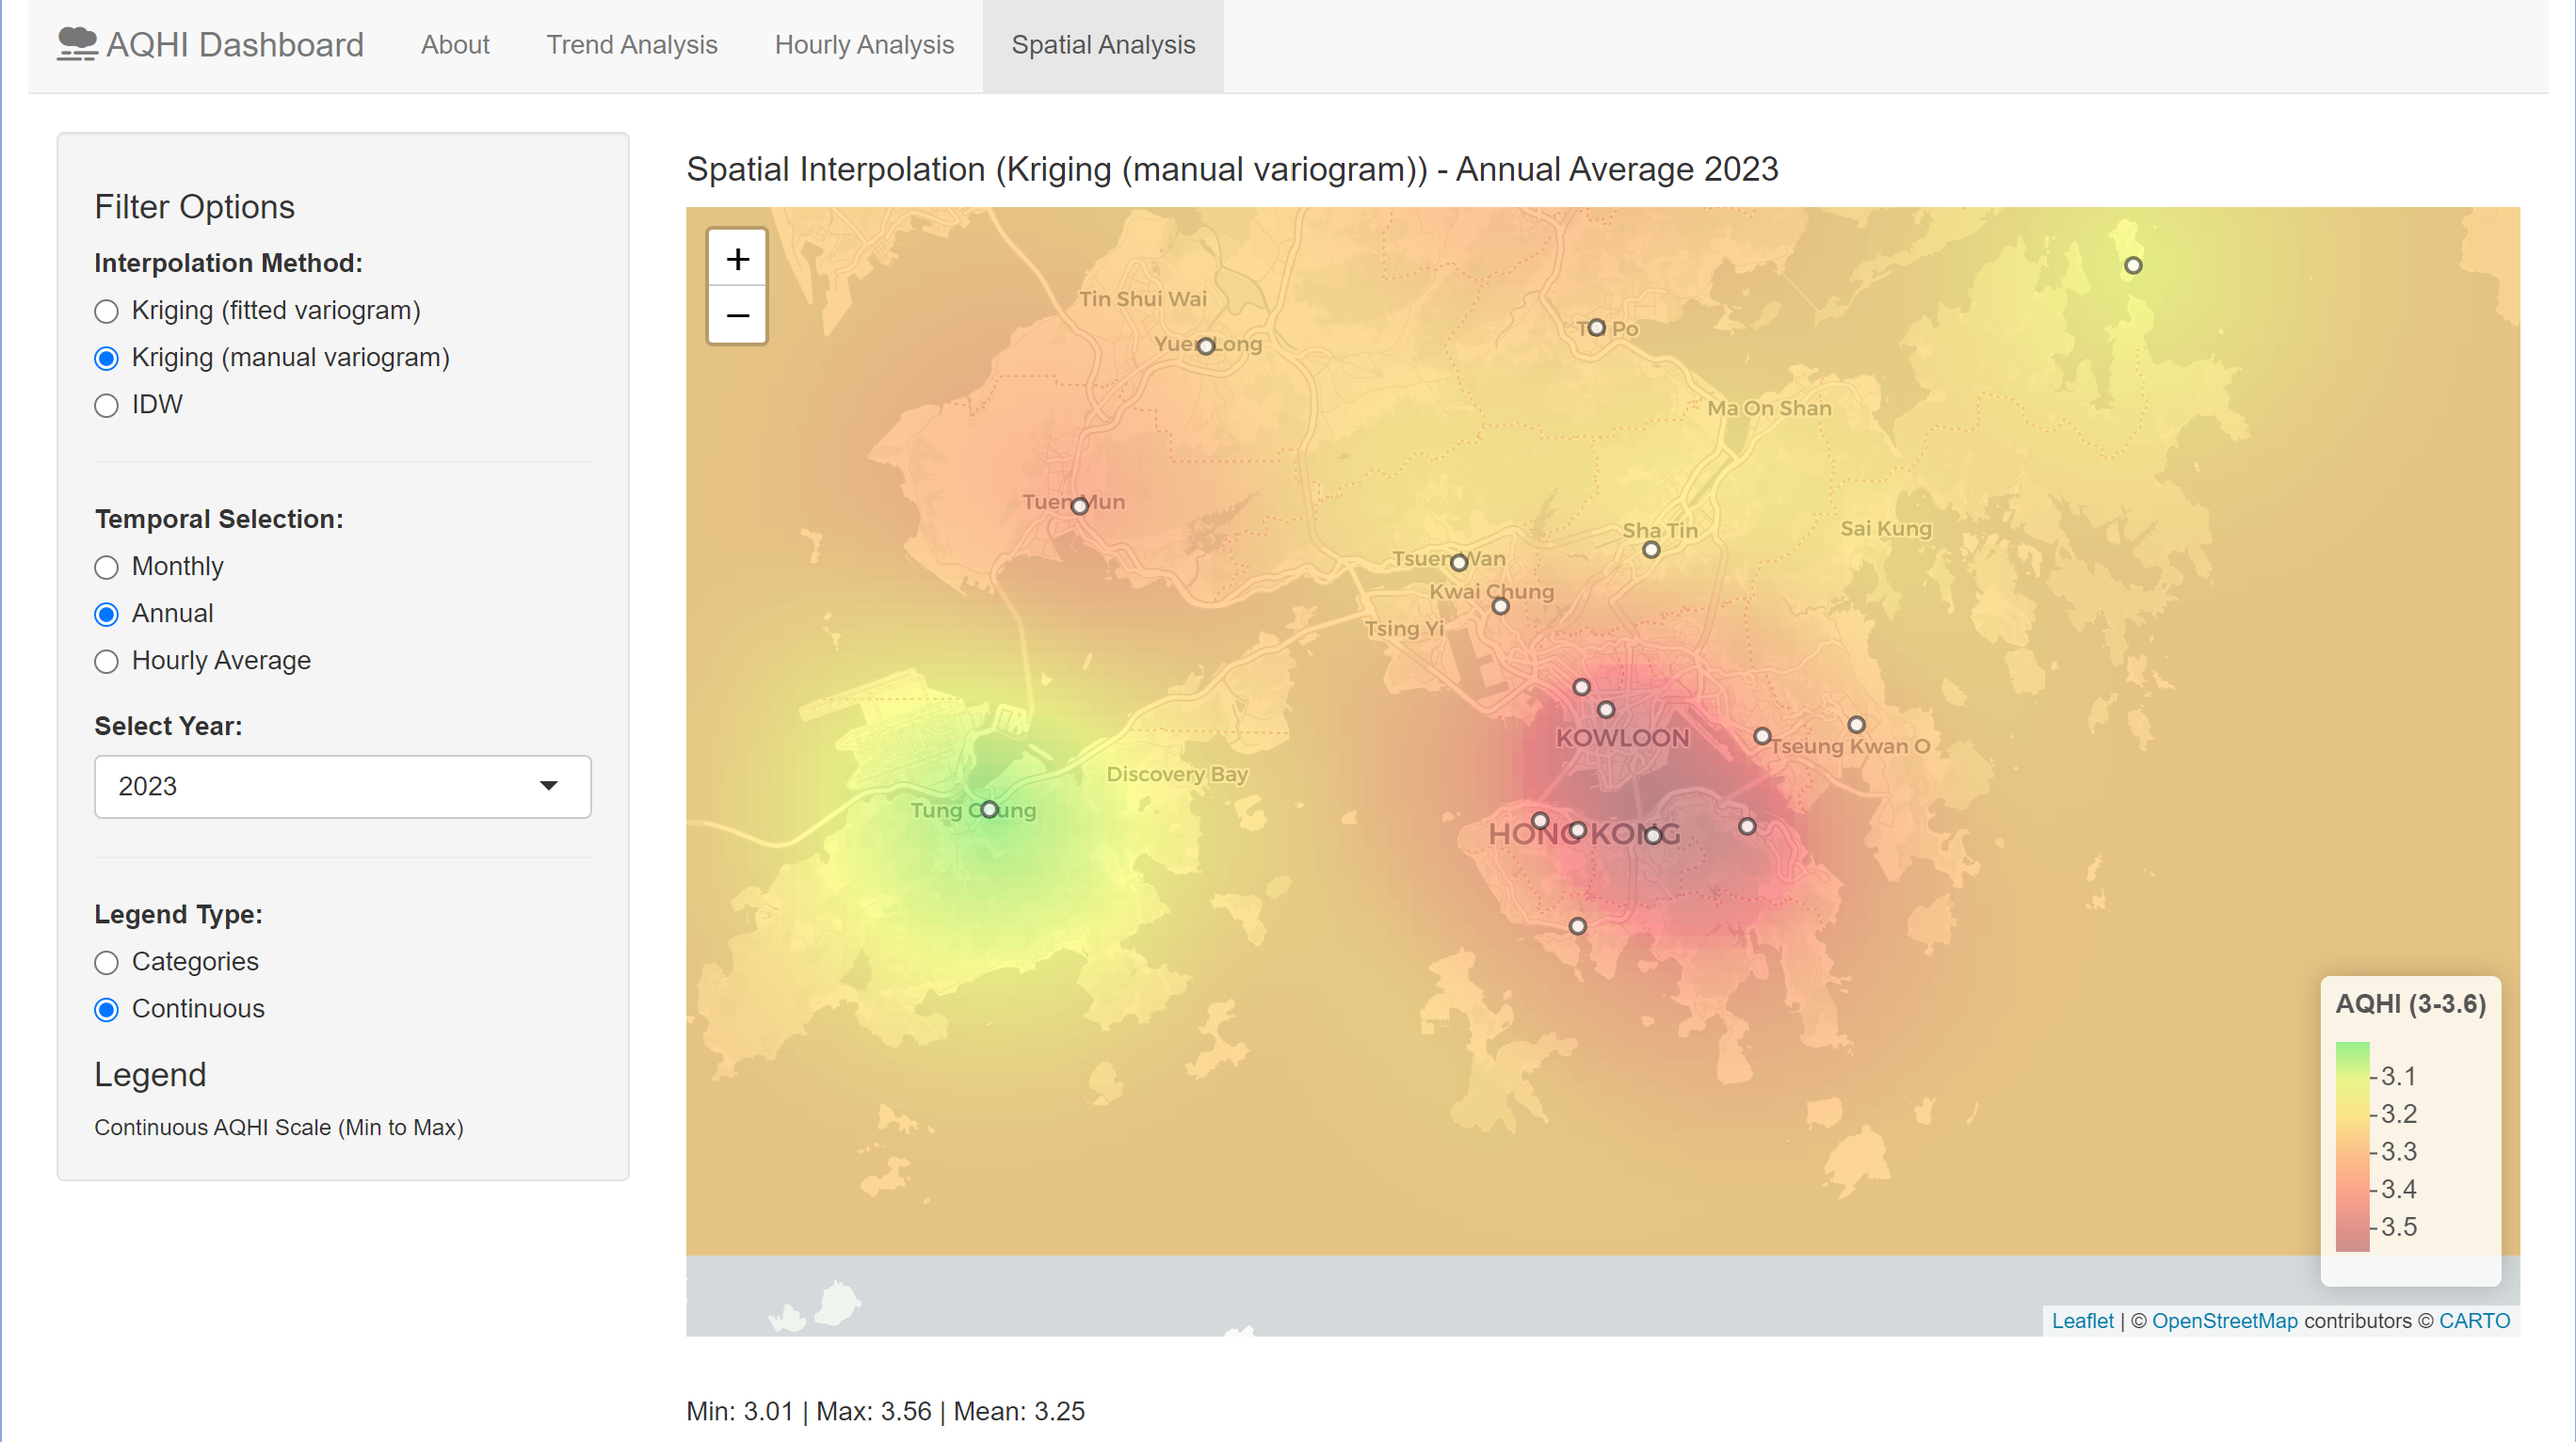
\includegraphics[width=\textwidth]{figures/spatial analysis.png}
                \caption{Spatial Analysis: Interpolated AQHI.}
                \label{fig:dashboard_spatial_analysis}
            \end{subfigure}
            \caption{Overview of the three main interactive components of the AQHI dashboard: Trend Analysis for temporal patterns, Hourly Analysis for diurnal cycles, and Spatial Analysis for geographic distribution of air quality.}
            \label{fig:dashboard_overview}
        \end{figure}

\section{Conclusion}

This project analyzed the spatio-temporal distribution of the Air Quality Health Index (AQHI) in Hong Kong using hourly observations from 2021 to 2025. A reproducible workflow was implemented including data preparation, temporal aggregation, spatial interpolation, and interactive visualization through a Shiny dashboard.\\
The temporal analysis revealed clear short-term and seasonal variation in AQHI values, while spatial differences between monitoring stations were comparatively moderate. Many stations exhibit similar AQHI ranges, and aggregation to monthly and annual averages further smooths spatial variability. As a result, only weak spatial structures are present in the data.\\
Because Kriging relies on spatial autocorrelation, the limited spatial variability reduces its advantage over simpler interpolation methods. For this reason, multiple approaches were implemented, including Inverse Distance Weighting (IDW) and two variants of Ordinary Kriging (automatically fitted and manually parameterized variograms). Comparing these methods improves interpretability and highlights methodological differences under weak spatial structure conditions.\\
Due to the relatively small differences between interpolated surfaces, a continuous color scale was added in addition to the categorical AQHI classification. This allows subtle spatial variations to remain visible while still supporting interpretation based on official risk categories.\\
Overall, the project demonstrates how multi-year environmental monitoring data can be integrated into a reproducible spatio-temporal analysis pipeline and communicated through interactive visualization. The developed dashboard enables flexible exploration of both temporal dynamics and spatial patterns of air quality in Hong Kong.


\section{Reproducibility and Repository}

All scripts and resources required to reproduce the analysis workflow and run the interactive dashboard are provided in the project repository available on \url{https://github.com/lraeuschel/AOSTD_final_assignment}. The repository contains the complete R scripts for data preparation, spatial interpolation, and visualization, as well as the Shiny application code.\\
Due to file size constraints, only the raw input datasets are stored in the repository. Therefore, the preprocessing and spatial interpolation scripts must be executed before running the dashboard in order to generate the intermediate processed datasets and raster layers used for visualization.\\
Detailed step-by-step instructions for setting up the environment and executing the workflow are documented in the README file within the repository. These instructions describe the required package dependencies and the recommended execution order of the scripts to ensure reproducibility of the results. If any issues arise during setup or execution, further questions can be directed to the author of this report.

\section{Usage of Artificial Intelligence}

Artificial intelligence tools were used in a supportive role during the preparation of this report. In particular, AI-based language assistance was applied to improve readability, grammar, and overall text clarity. Additionally, AI tools were used for occasional translations between German and English and for stylistic refinement of existing text passages.


% -------------------------
% Acknowledgments (optional)
% -------------------------
%\begin{acks}
%...
%\end{acks}

% -------------------------
% Literatur
% -------------------------


\bibliographystyle{ACM-Reference-Format}
\bibliography{references}

\end{document}